\subsubsection{Regressione}

Procediamo ora con l'analisi del grafico del dislivello $d$ in funzione della temperatura $\theta$.
In base ai dati da noi raccolti abbiamo ottenuto il seguente risultato, illustrato in figura (\ref{fig:dislivello_temperatura}).

\begin{SCfigure}[][p]
    \centering
    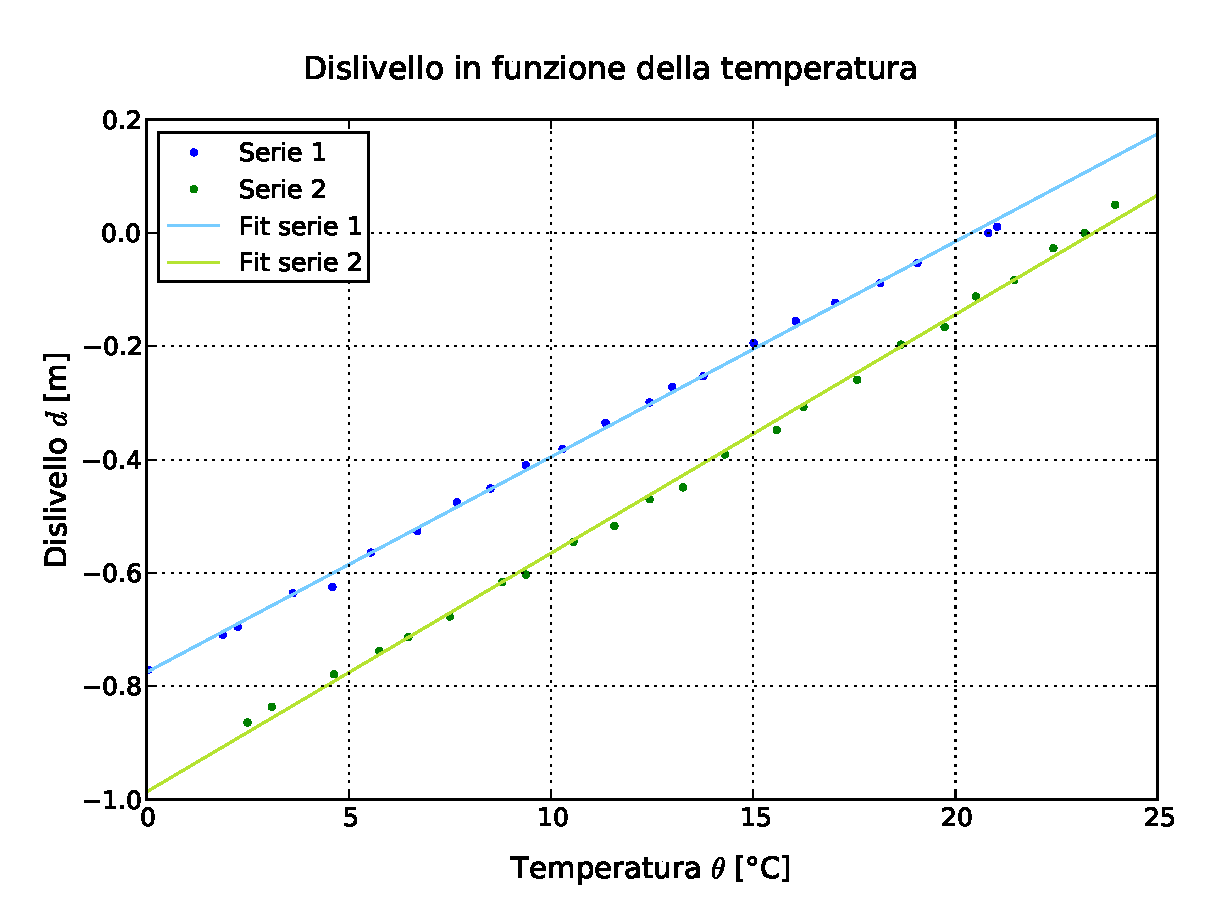
\includegraphics[width=120mm]{immagini/dislivello_temperatura.pdf}
    \caption{Il seguente grafico rappresenta}
    \label{fig:dislivello_temperatura}
\end{SCfigure}
%
Si vede che esiste una correlazione tra la temperatura $\theta$ e dislivello $d$ ed è anche approssimativamente lineare.
Con il metodo dei minimi quadrati, abbiamo quindi trovato la funzione lineare

\begin{equation}
	d \,=\, A + B\,\theta
	\label{h_theta}
\end{equation}
%
che meglio si adatta ai dati da noi raccolti. L'intera procedura qui descritta è stata
applicata ad entrambe le serie di dati separatamente.

Come primo passo abbiamo eseguito dei fit prelimiari sulle due serie di dati,
al fine di trasferire l'incertezza dalla temperatura al dislivello.
Per fare ciò occorre minimizzare la funzione

\begin{equation}
    \sum_{i=1}^{N} \frac{(d - A' - B'\theta)^2}{(\delta d)^2}
    \label{eq:min_quad}
\end{equation}
%
dove $N$ indica il numero di dati della serie, che sono 22 nella prima serie e 23 nella seconda.

Durante questa fase si è tenuto conto solamente dell'incertezza $\delta d$ sul dislivello. Per calcolare i minimi
di (\ref{eq:min_quad}) si sono usate le formule:

\begin{equation}
    \left(
    \begin{array}{c}
        A' \\
        B'
    \end{array} 
    \right)
    =
    M^{-1}
    \left(
    \begin{array}{c}
        \sum d/(\delta d)^2 \\[2mm]
        \sum (\theta d)/(\delta d)^2
    \end{array} 
    \right)
    \qquad 
    \text{dove}
    \quad
    M =
    \left(
    \begin{array}{c c}
        \sum 1/(\delta d)^2 & \sum \theta/(\delta d)^2 \\[2mm]
        \sum \theta/(\delta d)^2 & \sum \theta^2/(\delta d)^2
    \end{array} 
    \right)
    \label{eq:A_e_B}
\end{equation}
%
dove tutte le sommatorie vanno da 1 a $N$ e non si è scritto l'indice per motivi di spazio. Mediante le regole
di propagazione degli errori si può calcolare che le incertezze su $A'$ e $B'$ valgono

\begin{equation}
    \delta A' \,=\, \sqrt{\frac{\sum \theta^2/(\delta d)^2}{\det(M)}}
    \qquad
    \delta B' \,=\, \sqrt{\frac{\sum 1/(\delta d)^2}{\det(M)}}
    \label{eq:dA_e_dB}
\end{equation}

Una volta calcolato $B'$ si è trasferito l'errore dalla temperatura al dislivello nel seguente modo

\begin{equation}
    \delta d\ped{tot} = \sqrt{\delta d^2 + (B'\delta \theta)^2}
\end{equation}
%
Infine si è minimizzata nuovamente la (\ref{eq:min_quad}), sempre tramite le formule (\ref{eq:A_e_B}) e (\ref{eq:dA_e_dB})
dovutamente modificate, utilizzando però $\delta d\ped{tot}$ invece che $\delta d$.
%
Si sono così ricavati i valori definitivi $A$ e $B$. La procedura è stata applica ad entrambe le serie di dati.
Le rette ottenute sono riportate nel grafico in figura \ref{fig:dislivello_temperatura}, assieme ai dati delle due serie.
Nella seguente tabella sono riportati i risulatati di fit preliminari e finali per le due serie.

\begin{center}
    \small
    \begin{tabular}{l c c c c c c c c c}
        \toprule
        & $A'$ & $B'$ & $\delta A'$ & $\delta B'$ &
        $\delta d\ped{tot}$ & $A$ & $B$ & $\delta A$ & $\delta B$ \\
        & [cm] & [\si{\centi\meter\per\celsius}] &  [cm] & [\si{\centi\meter\per\celsius}] &
        [cm] & [cm] & [\si{\centi\meter\per\celsius}] & [cm] & [\si{\centi\meter\per\celsius}] \\
        \midrule
        Serie 1 & -77.57 & 3.804 & 0.02 & 0.001 & 0.04 & -77.57 & 3.804 & 0.02 & 0.001 \\
        Serie 2  & -98.68 & 4.215 & 0.02 & 0.001 & 0.04 & -98.68 & 4.215 & 0.02 & 0.001 \\
        \bottomrule
    \end{tabular}
\end{center}

Nella tabella è riportato anche il $\delta d\ped{tot}$ con l'aggiunta dell'incertezza trasferita. Chiaramente, l'incertezza trasferita è
trascurabile poiché il valore $\delta d\ped{tot}$ è identico a $\delta d$. Anche le incertezze sui parametri $A'$, $B'$, $A$ e $B$
non hanno subito variazioni tra i fit preliminari e le regressioni definitive.

I valori ottenuti fit finali sono compatibili con quelli ricavati dalle regressioni preliminari; infatti tutti i parametri
sono uguali entro l'incertezza per entrambe le serie di dati.
